\documentclass{article}
\usepackage{amsmath}
\usepackage{amssymb}
\usepackage{graphicx}
\usepackage[margin=1in]{geometry}
\usepackage{hyperref}
\usepackage{caption}
\usepackage{float}
\graphicspath{{images/}}
\hypersetup{
  colorlinks=true,
  urlcolor=blue,
}
\begin{document}

\title{A Generating Function Problem}
\author{Aresh Pourkavoos}
\maketitle

Problem:
\begin{align*}
  f(x, 0) &= \frac{e^x-1}{x} \\
  f(x, y) &= \frac{\partial f}{\partial x}(x, y)+\frac{\partial f}{\partial y}(x, y)
\end{align*}
Solution: Define
\[A(j, k) = \frac{\partial^{j+k} f}{\partial x^j \partial y^k}(0, 0)\]
Get Taylor series of base case:
\[f(x, 0)
= \frac{1}{x} \left(\sum_{i=0}^\infty \frac{x^i}{i!}-1\right)
= \frac{1}{x} \left(\sum_{i=1}^\infty \frac{x^i}{i!}\right)
= \frac{1}{x} \left(\sum_{i=0}^\infty \frac{x^{i+1}}{(i+1)!}\right)
= \sum_{i=0}^\infty \frac{x^i}{(i+1)!}\]
Find partial derivatives wrt $x$:
\[A(j, 0)
= \frac{\partial^j f}{\partial x^j} \sum_{i=0}^\infty \frac{x^i}{(i+1)!}
= \frac{\partial^j f}{\partial x^j} \frac{x^j}{(j+1)!}
= \frac{j!}{(j+1)!}
= \frac{1}{j+1}\]
Use diffeq to establish recurrence relation on $A$:
\begin{align*}
  A(j, k)
  &= \frac{\partial^{j+k} f}{\partial x^j \partial y^k}(0, 0) \\
  &= \frac{\partial}{\partial x}\left(\frac{\partial^{j+k} f}{\partial x^j \partial y^k}\right)(0, 0)
  + \frac{\partial}{\partial y}\left(\frac{\partial^{j+k} f}{\partial x^j\partial y^k}\right)(0, 0) \\
  &= \frac{\partial^{j+k+1} f}{\partial x^{j+1} \partial y^k}(0, 0)
  + \frac{\partial^{j+k+1} f}{\partial x^j \partial y^{k+1}}(0, 0) \\
  &= A(j+1, k)+A(j, k+1)
\end{align*}
Rearrange to compute higher values of $k$:
\[A(j, k+1) = A(j, k)-A(j+1, k)\]
These are sufficient to determine all $A(j, k)$,
which may be found by computation and guess-and-check:
\[A(j, k) = \frac{j!k!}{(j+k+1)!} = B(j+1, k+1)\]
where B is the beta function. Construct 2D Taylor series:
\begin{align*}
  f(x, y)
  &= \sum_{j=0}^\infty \sum_{k=0}^\infty A(j, k) \frac{x^jy^k}{j!k!} \\
  &= \sum_{j=0}^\infty \sum_{k=0}^\infty \frac{j!k!}{(j+k+1)!} \frac{x^jy^k}{j!k!} \\
  &= \sum_{j=0}^\infty \sum_{k=0}^\infty \frac{x^jy^k}{(j+k+1)!} \\
  &= \sum_{n=0}^\infty \sum_{j+k=n} \frac{x^jy^k}{(j+k+1)!} \\
  &= \sum_{n=0}^\infty \frac{1}{(n+1)!}\sum_{j+k=n} x^jy^k \\
  &= \sum_{n=0}^\infty \frac{1}{(n+1)!}\frac{x^{n+1}-y^{n+1}}{x-y} \\
  &= \frac{1}{x-y}\left(
  \sum_{n=0}^\infty \frac{x^{n+1}}{(n+1)!}-\sum_{n=0}^\infty \frac{y^{n+1}}{(n+1)!}
  \right) \\
  &= \frac{1}{x-y}((e^x-1)-(e^y-1)) \\
  &= \frac{e^x-e^y}{x-y}
\end{align*}
Check answer:
\[f(x, 0) = \frac{e^x-e^0}{x-0} = \frac{e^x-1}{x}\]
\begin{align*}
  \frac{\partial f}{\partial x} &= \frac{e^x(x-y)-(e^x-e^y)}{(x-y)^2} \\
  \frac{\partial f}{\partial y} &= \frac{-e^y(x-y)+(e^x-e^y)}{(x-y)^2} \\
  \frac{\partial f}{\partial x}+\frac{\partial f}{\partial y} &= \frac{(e^x-e^y)(x-y)}{(x-y)^2} \\
  &= \frac{e^x-e^y}{(x-y)} \\
  &= f(x, y)
\end{align*}
\newpage
3D variant:
\[A(j, k, l) = \frac{j!k!l!}{(j+k+l+2)!} = B(j+1, k+1, l+1)
= \frac{\partial^{j+k+l}f}{\partial x^j \partial y^k \partial z^l}\]
Diffeq:
\[
f(x, y, z)
= \frac{\partial f}{\partial x}(x, y, z)
+ \frac{\partial f}{\partial y}(x, y, z)
+ \frac{\partial f}{\partial z}(x, y, z)
\]
Solution:
\begin{align*}
  f(x, y, z) &= \sum_{j=0}^\infty\sum_{k=0}^\infty\sum_{l=0}^\infty\frac{x^jy^kz^l}{(j+k+l+2)!} \\
  &= \sum_{n=0}^\infty\mathop{\sum\sum}_{j+k+l=n}\frac{x^jy^kz^l}{(j+k+l+2)!} \\
  &= \sum_{n=0}^\infty\frac{1}{(n+2)!}\mathop{\sum\sum}_{j+k+l=n}x^jy^kz^l \\
  &= \sum_{n=0}^\infty\frac{1}{(n+2)!}\frac{(y-z)x^{n+2}+(z-x)y^{n+2}+(x-y)z^{n+2}}{(z-y)(x-z)(y-x)} \\
  &= \frac{1}{(z-y)(x-z)(y-x)}\left(
  (y-z)\sum_{n=0}^\infty\frac{x^{n+2}}{(n+2)!} +
  (z-x)\sum_{n=0}^\infty\frac{y^{n+2}}{(n+2)!} +
  (x-y)\sum_{n=0}^\infty\frac{z^{n+2}}{(n+2)!}
  \right) \\
  &= \frac{1}{(z-y)(x-z)(y-x)}((y-z)(e^x-1-x)+(z-x)(e^y-1-y)+(x-y)(e^z-1-z)) \\
  &= \frac{e^x(y-z)+e^y(z-x)+e^z(x-y)}{(z-y)(x-z)(y-x)} \\
  &= -\frac{e^x}{(x-z)(y-x)}-\frac{e^y}{(z-y)(y-x)}-\frac{e^z}{(z-y)(x-z)} \\
  &= \frac{e^x}{(x-y)(x-z)}+\frac{e^y}{(y-x)(y-z)}+\frac{e^z}{(z-x)(z-y)}
\end{align*}
Check answer:
\begin{align*}
  \frac{\partial f}{\partial x}(x, y, z)
  &= \frac{\partial}{\partial x}\left(\frac{e^x}{(x-y)(x-z)}+\frac{e^y}{(y-x)(y-z)}+\frac{e^z}{(z-x)(z-y)}\right) \\
  &= \frac{\partial}{\partial x}\frac{e^x}{(x-y)(x-z)}+\frac{\partial}{\partial x}\frac{e^y}{(y-x)(y-z)}+\frac{\partial}{\partial x}\frac{e^z}{(z-x)(z-y)} \\
  &= \frac{\left(\frac{\partial}{\partial x}e^x\right)(x-y)(x-z)-e^x\left(\frac{\partial}{\partial x}((x-y)(x-z))\right)}{(x-y)^2(x-z)^2w}+\frac{e^y}{(y-x)^2(y-z)}+\frac{e^z}{(z-x)^2(z-y)} \\
  &= \frac{e^x(x-y)(x-z)-e^x((x-y)+(x-z))}{(x-y)^2(x-z)^2}+\frac{e^y}{(y-x)^2(y-z)}+\frac{e^z}{(z-x)^2(z-y)} \\
  &= \frac{e^x}{(x-y)(x-z)}-\frac{e^x}{(x-y)(x-z)^2}-\frac{e^x}{(x-y)^2(x-z)}+\frac{e^y}{(y-x)^2(y-z)}+\frac{e^z}{(z-x)^2(z-y)} \\
  \frac{\partial f}{\partial y}(x, y, z)
  &= \frac{e^x}{(x-y)^2(x-z)}+\frac{e^y}{(y-x)(y-z)}-\frac{e^y}{(y-x)(y-z)^2}-\frac{e^y}{(y-x)^2(y-z)}+\frac{e^z}{(z-x)(z-y)^2} \\
  \frac{\partial f}{\partial z}(x, y, z)
  &= \frac{e^x}{(x-y)(x-z)^2}+\frac{e^y}{(y-x)(y-z)^2}+\frac{e^z}{(z-x)(z-y)}-\frac{e^z}{(z-x)(z-y)^2}-\frac{e^z}{(z-x)^2(z-y)}
\end{align*}
Each term with quadratic denominator only appears once across all partials \\
Each term with cubic denominator appears twice across all partials,
once positive and once negative \\
When added, cubic terms cancel and quadratics remain to form $f(x, y, z)$
\newpage
$N$D solution:
\[
f(x_1, \ldots, x_N) =
\sum_{I=1}^N\frac{e^{x_I}}{\prod\limits_{J \neq I}(x_I-x_J)}
%% \frac{e^{x_1}}{(x_1-x_2)\cdots(x_1-x_N)}
%% +\frac{e^{x_2}}{(x_2-x_1)\cdots(x_2-x_N)}
%% +\cdots
%% +\frac{e^{x_N}}{(x_N-x_1)(x_N-x_2)\cdots}
\]
$I \neq K$: Define
\[T(I, K) = \frac{\partial}{\partial x_K} \frac{e^{x_I}}{\prod\limits_{J \neq I}(x_I-x_J)}
= \frac{e^{x_I}}{(x_I-x_K)\prod\limits_{J \neq I}(x_I-x_J)}\]
Partial derivative of remaining terms ($I=K$):
\begin{align*}
  \frac{\partial}{\partial x_K} \frac{e^{x_K}}{\prod\limits_{J \neq K}(x_K-x_J)}
  &= \frac{\frac{\partial}{\partial x_K}e^{x_K}}{\prod\limits_{J \neq K}(x_K-x_J)}-\frac{e^{x_K}\frac{\partial}{\partial x_K}\prod\limits_{J \neq K}(x_K-x_J)}{\prod\limits_{J \neq K}(x_K-x_J)^2} \\
  &= \frac{e^{x_K}}{\prod\limits_{J \neq K}(x_K-x_J)}-\frac{e^{x_K}\sum\limits_{L \neq K}\prod\limits_{J \not\in \{K, L\}}(x_K-x_J)}{\prod\limits_{J \neq K}(x_K-x_J)^2} \\
  &= \frac{e^{x_K}}{\prod\limits_{J \neq K}(x_K-x_J)}-\sum_{L \neq K}\frac{e^{x_K}}{(x_K-x_L)\prod\limits_{J \neq K}(x_K-x_J)} \\
  &= \frac{e^{x_K}}{\prod\limits_{J \neq K}(x_K-x_J)}-\sum_{L \neq K}T(K, L)
\end{align*}
Overall derivative for given $x_K$:
\begin{align*}
  \frac{\partial f}{\partial x_K}(x_1, \ldots, x_N)
  &= \frac{\partial}{\partial x_K} \sum_{I=1}^N \frac{e^{x_I}}{\prod\limits_{J \neq I}(x_I-x_J)} \\
  &= \frac{\partial}{\partial x_K} \frac{e^{x_K}}{\prod\limits_{J \neq K}(x_K-x_J)} + \sum_{I \neq K} \frac{\partial}{\partial x_K} \frac{e^{x_I}}{\prod\limits_{J \neq I}(x_I-x_J)} \\
  &= \frac{e^{x_K}}{\prod\limits_{J \neq K}(x_K-x_J)}-\sum\limits_{L \neq K}T(K, L)+\sum_{I \neq K}T(I, K)
\end{align*}
Sum of all partials:
\begin{align*}
  \sum_{K=1}^N\frac{\partial f}{\partial x_K}(x_1, \ldots, x_N)
  &= \sum_{K=1}^N\left(\frac{e^{x_K}}{\prod\limits_{J \neq K}(x_K-x_J)}-\sum\limits_{L \neq K}T(K, L)+\sum_{I \neq K}T(I, K)\right) \\
  &= \sum_{K=1}^N\frac{e^{x_K}}{\prod\limits_{J \neq K}(x_K-x_J)}-\sum_{K=1}^N\sum\limits_{L \neq K}T(K, L)+\sum_{K=1}^N\sum_{I \neq K}T(I, K) \\
  &= \sum_{K=1}^N\frac{e^{x_K}}{\prod\limits_{J \neq K}(x_K-x_J)} \\
  &= f(x_1, \ldots, x_N)
\end{align*}
Remains to be shown that derivative is the multivariate beta function:
\[\frac{\partial^{k_1+\ldots+k_K}f}{\partial x_1^{k_1}\ldots\partial x_N^{k_n}}
= \frac{k_1! \ldots k_N!}{(k_1+\ldots+k_N+N-1)!}\]
\newpage
Lemma 1:
\[\prod_{1 \leq i < j \leq n} (x_j-x_i) = \sum_{\sigma \in S_n}\left(\text{sgn}(\sigma)\prod_{k=1}^nx_k^{\sigma_k-1}\right),\]
where $S_n$ is the set of permutations of the sequence $(1, \ldots, n)$.
Ex for $n=3$:
\begin{align*}
  (x_2-x_1)(x_3-x_1)(x_3-x_2)
  &= x_1^0x_2^1x_3^2-x_1^0x_2^2x_3^1-x_1^1x_2^0x_3^2+x_1^1x_2^2x_3^0-x_1^2x_2^0x_3^1+x_1^2x_2^1x_3^0 \\
  &= x_2x_3^2-x_2^2x_3-x_1x_3^2+x_1x_2^2-x_1^2x_3+x_1^2x_2
\end{align*}
Proof (sketch): Setting $x_i=x_j$ for any $1 \leq i < j \leq n$ makes the RHS 0
because the permutations may be placed into canceling pairs
where $\sigma_i$ and $\sigma_j$ switch values.
The product is the same for each, but the sign is flipped.
Thus the RHS is divisible by $x_j-x_i$.
Since $x_j-x_i$ share no factors with each other,
the RHS is divisible by their product, i.e. the LHS.
Since the LHS and RHS are both of degree $\binom{n}{2}$,
they can only differ by a constant factor.
On the RHS, the identity permutation has the term $\prod\limits_{k=1}^nx_k^k$
with coefficient 1 (since the identity permutation is even).
On the LHS, the only way to make this term
is to choose $x_n$ in the $n-1$ terms where it appears (all positive),
then $x_{n-1}$ in the $n-2$ terms of the remaining ones (again, all positive),
etc. until $x_2$ is chosen from $x_2-x_1$.
Thus the coefficient on the LHS is also 1,
so the constant factor relating it and the RHS is 1,
so they are equal.

The value of either side is the determinant of the Vandermonde matrix
\[
V=
\begin{pmatrix}
  1 & x_1 & \ldots & x_1^{n-1} \\
  1 & x_2 & \ldots & x_2^{n-1} \\
  \vdots & \vdots & \ddots & \vdots \\
  1 & x_n & \ldots & x_n^{n-1}
\end{pmatrix},
\]
which may be seen from the definition of the determinant and the RHS. \\

Lemma 2:
\[\prod_{1 \leq i < j \leq n} (x_j-x_i)
= \sum_{l=1}^n\left((-1)^{n+l}x_l^{n-1}\prod_{\substack{1 \leq i < j \leq n \\ i \neq l \neq j}}(x_j-x_i)\right).\]
Proof: May be shown by separating the $n!$ terms of the LHS into $n$ sets of $(n-1)!$
by whichever $x_l$ is raised to $n-1$, factoring out $x_l^{n-1}$,
noting that the remaining exponents are a permutation of $(1, \ldots, n-2)$,
and applying Lemma 1 in reverse,
factoring in the power of $-1$ to account for the change in sign of the permutation. \\
Alternatively, perform cofactor expansion on the last column of the Vandermonde matrix,
noting that each of the $n$ minors is another Vandermonde matrix. \\

Theorem:
\[\prod_{1 \leq i < j \leq n} (x_j-x_i) \sum_{p_1+\ldots+p_n=k} \prod_{l=1}^n x_l^{p_l} = 
\sum_{l=1}^n\left((-1)^{n+l}x_l^{n-1+k}\prod_{\substack{1 \leq i < j \leq n \\ i \neq l \neq j}}(x_j-x_i)\right).
\]
Proof: First, note that the RHS is the same as that of Lemma 2,
but with $k$ added to the exponent of $x_l^{n-1}$.
The product in the RHS may be written as a determinant as per Lemma 1,
making the entire expression a cofactor expansion of the determinant of
\[
W=
\begin{pmatrix}
  1 & \ldots & x_1^{n-2} & x_1^{n-1+k} \\
  \vdots & \ddots & \vdots & \vdots \\
  1 & \ldots & x_{n-1}^{n-2} & x_{n-1}^{n-1+k} \\
  1 & \ldots & x_n^{n-2} & x_n^{n-1+k}
\end{pmatrix},
\]
which is the Vandermonde matrix, but with $k$ added to the exponents of the last column.
Since matrix multiplication respects the determinant,
it would suffice to find a matrix $U$ such that $VU=W$ and
\[\det(U) = \sum_{p_1+\ldots+p_n=k} \prod_{l=1}^n x_l^{p_l}.\]
Since all columns of $W$ but the last are the same as those of $V$,
the corresponding columns of $U$ are the same as those of the identity matrix.
Thus we only need to find the last column,
i.e. some vector $\vec{u}$ such that
\[
V\vec{u} =
\begin{pmatrix}
  x_1^{n-1+k} \\
  \vdots \\
  x_{n-1}^{n-1+k} \\
  x_n^{n-1+k}
\end{pmatrix}.
\]
Furthermore, since $U$ is upper triangular,
its determinant is the product of its diagonal entries,
and since all of those entries except the last are 1,
it suffices to show that the last entry of $\vec{u}$ is the desired determinant.

Used sympy to compute $\vec{u}$ for a few values of $n$ and $k$: \\
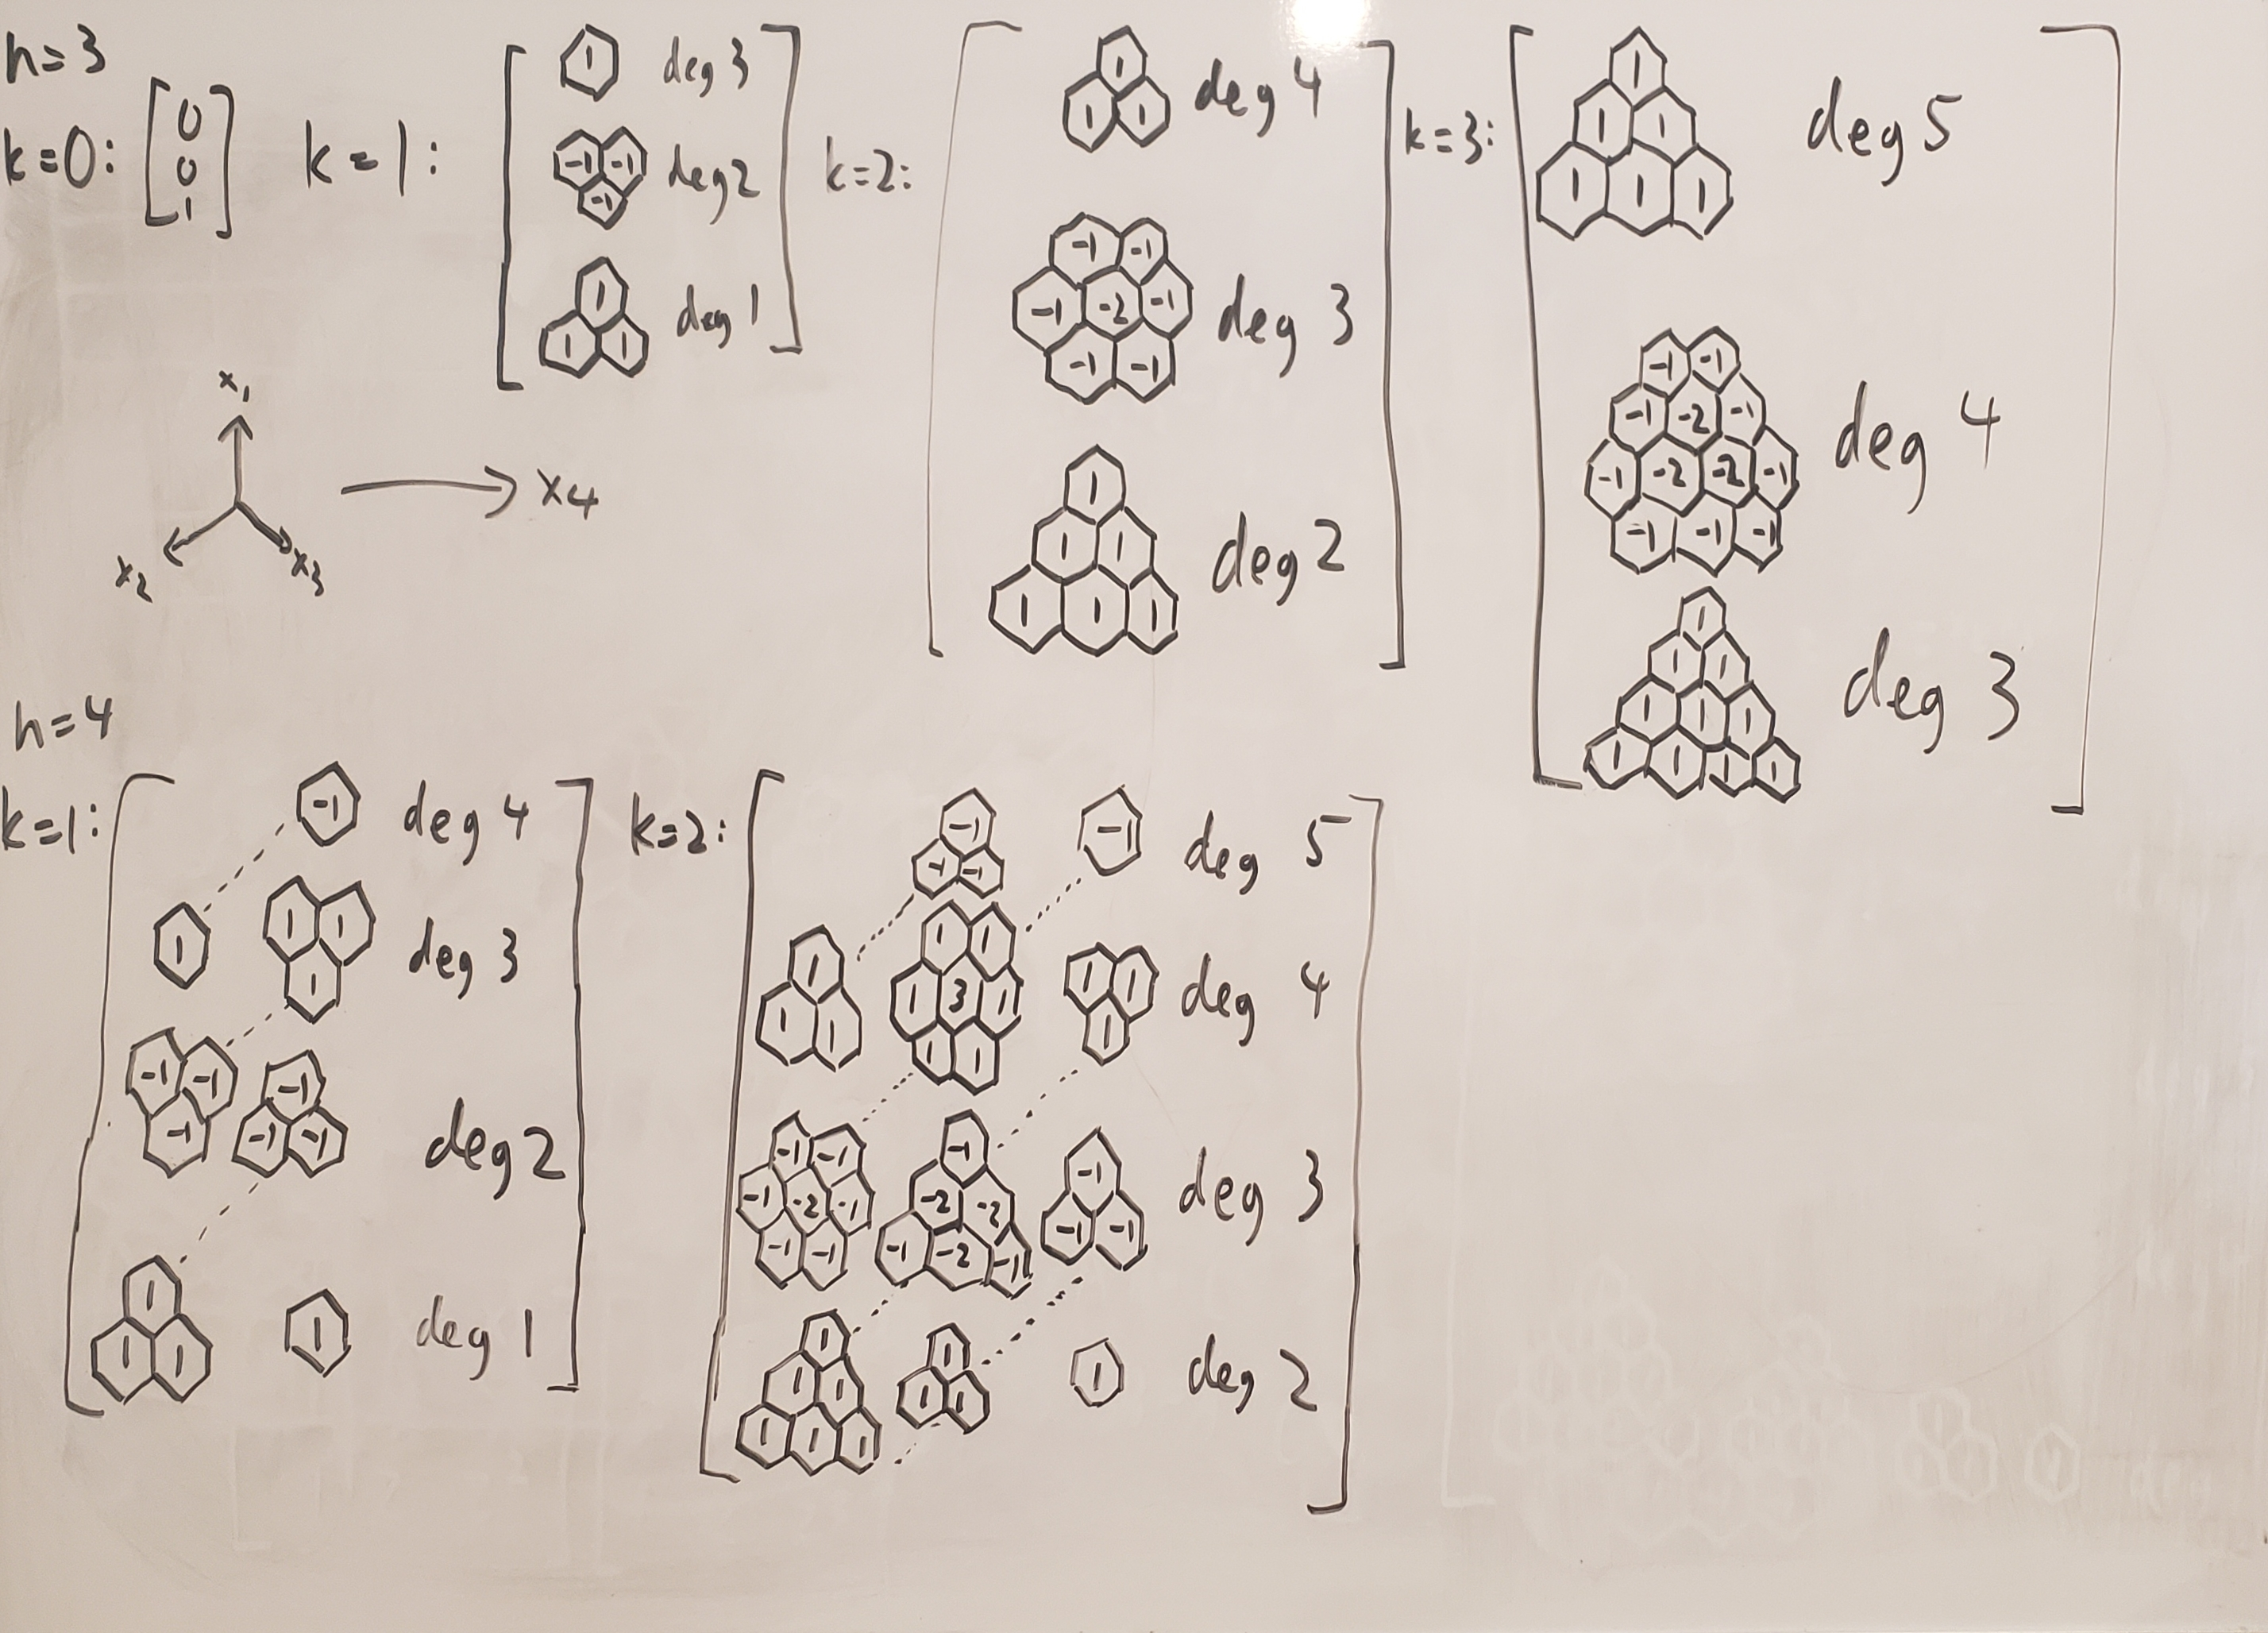
\includegraphics[width=0.5\linewidth]{u2.jpg}
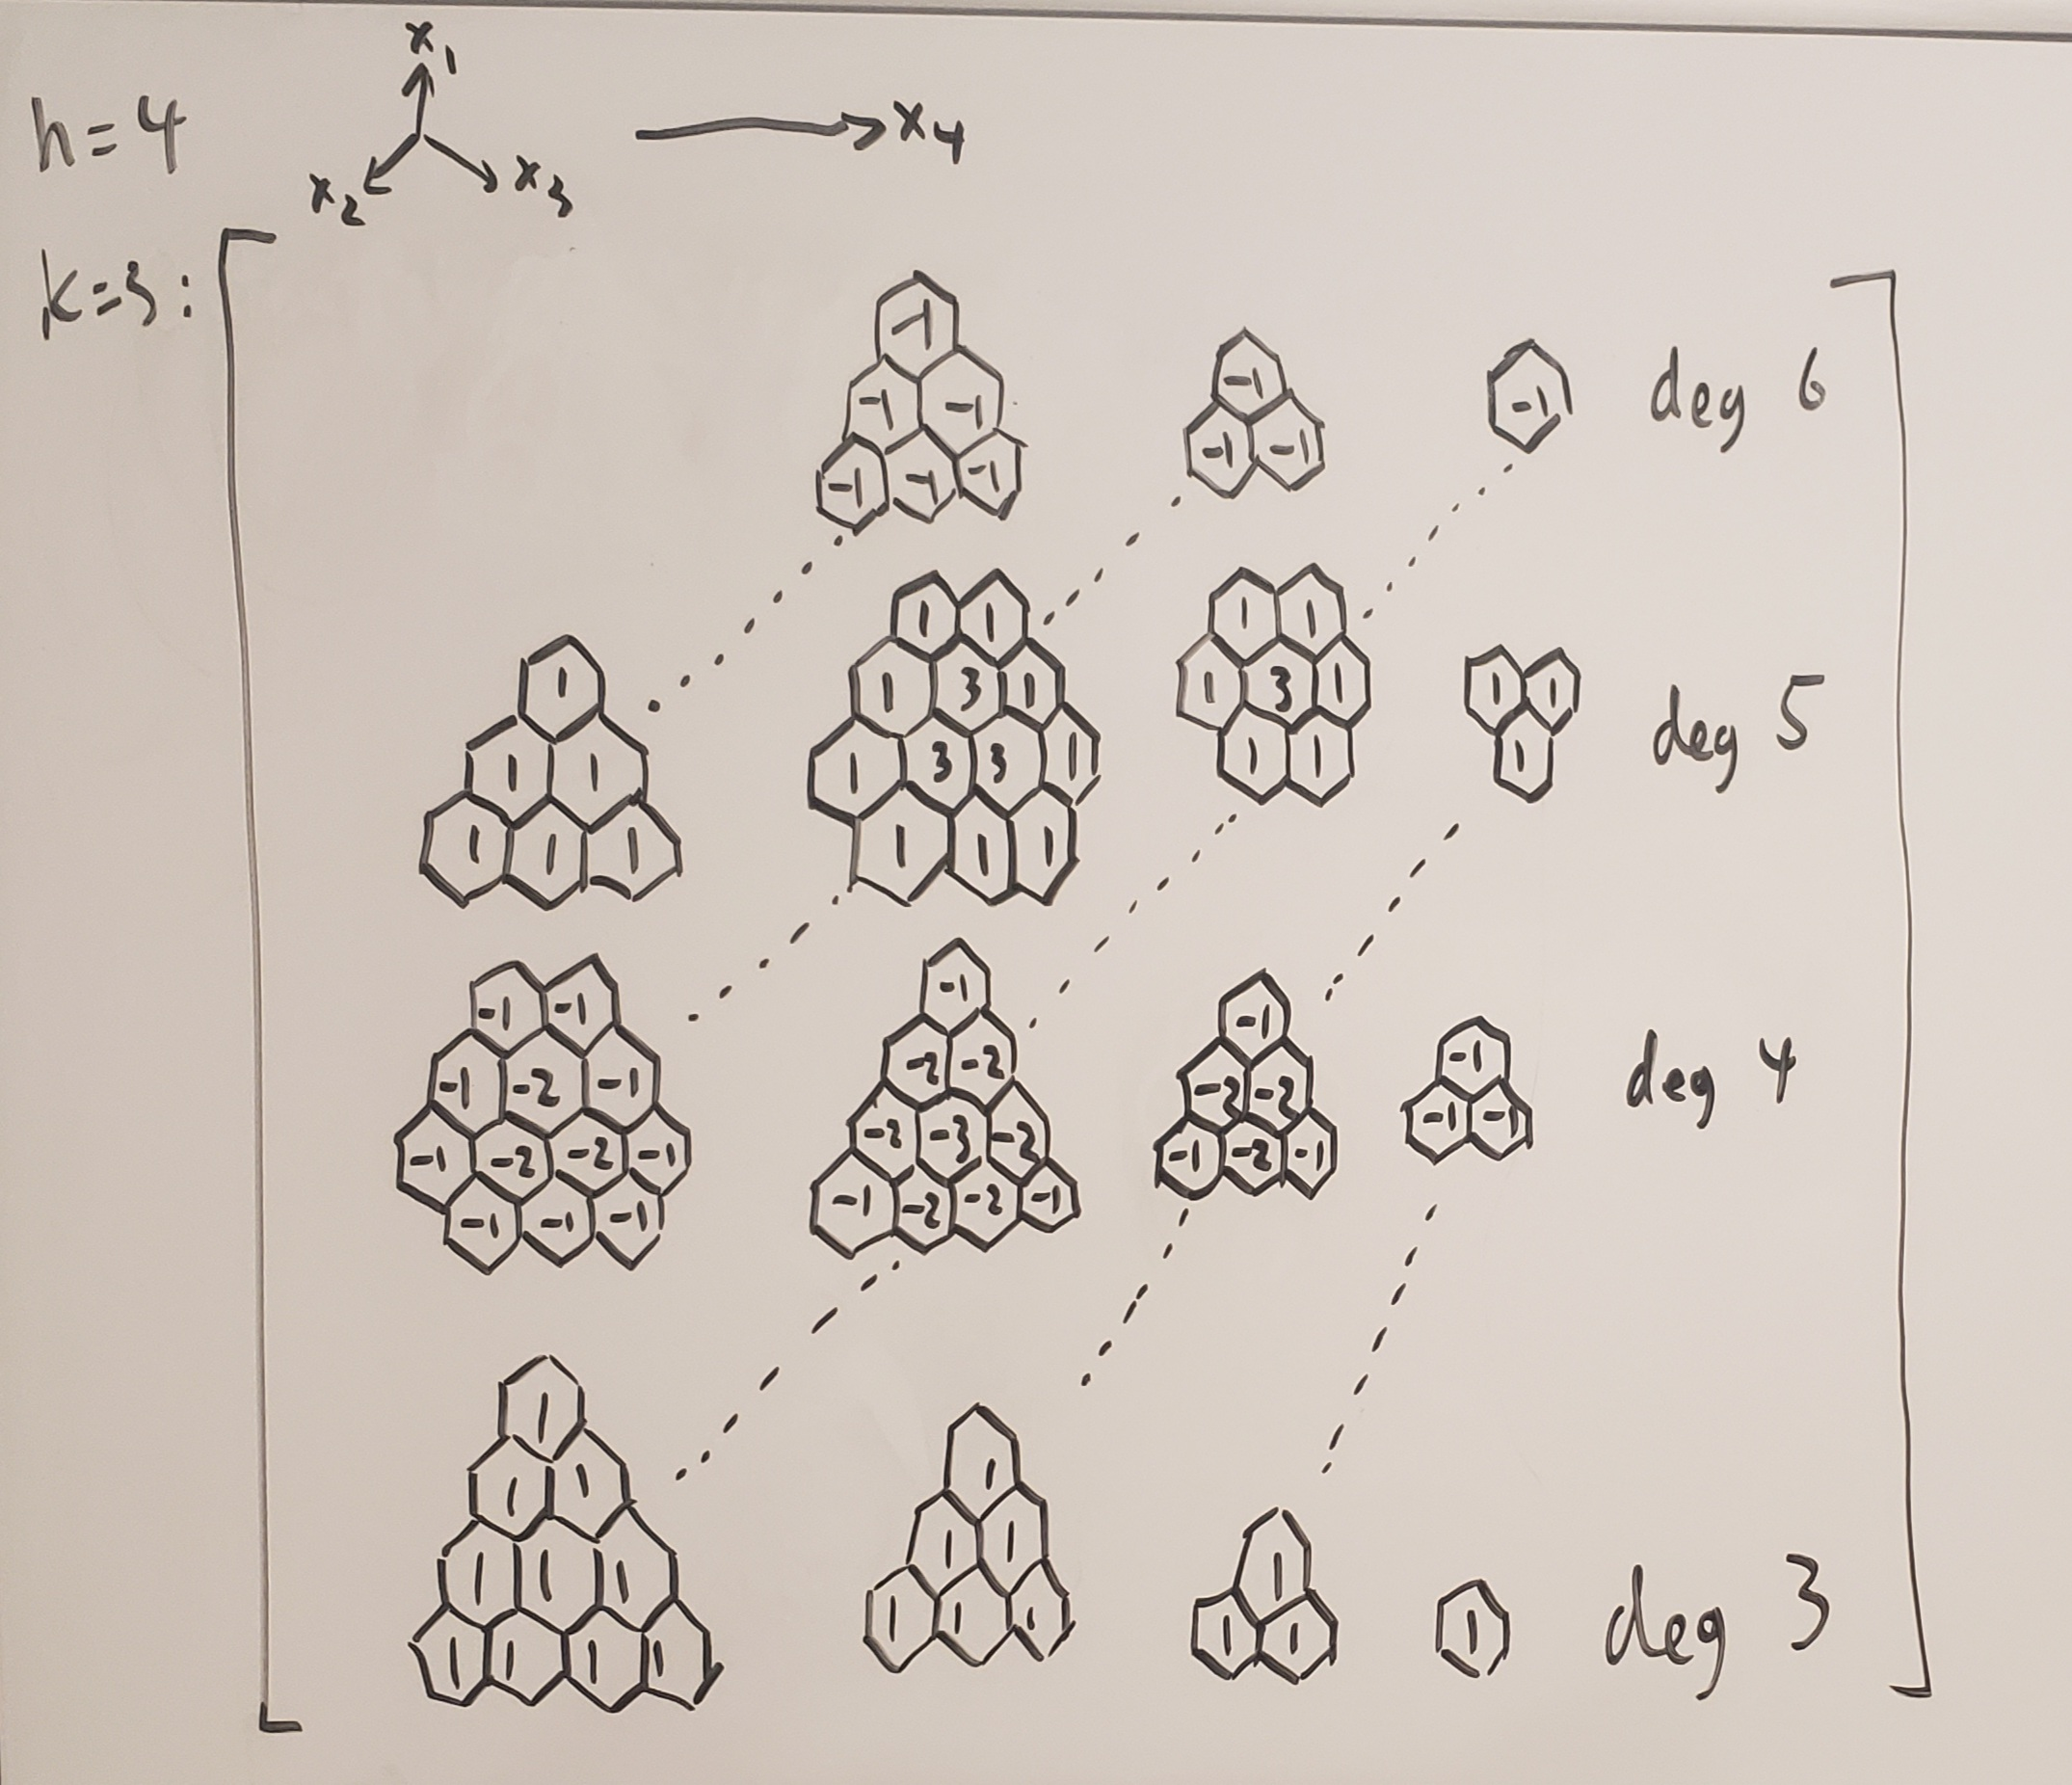
\includegraphics[width=0.5\linewidth]{u1.jpg}

First entry of vector seems to be a simplex 1 unit smaller than the last \\
Diagonals for $n=4$ sum to 0 (except bottom right)


\end{document}
